\documentclass[tikz, border=2pt]{standalone}
\usepackage{amsmath}

\begin{document}
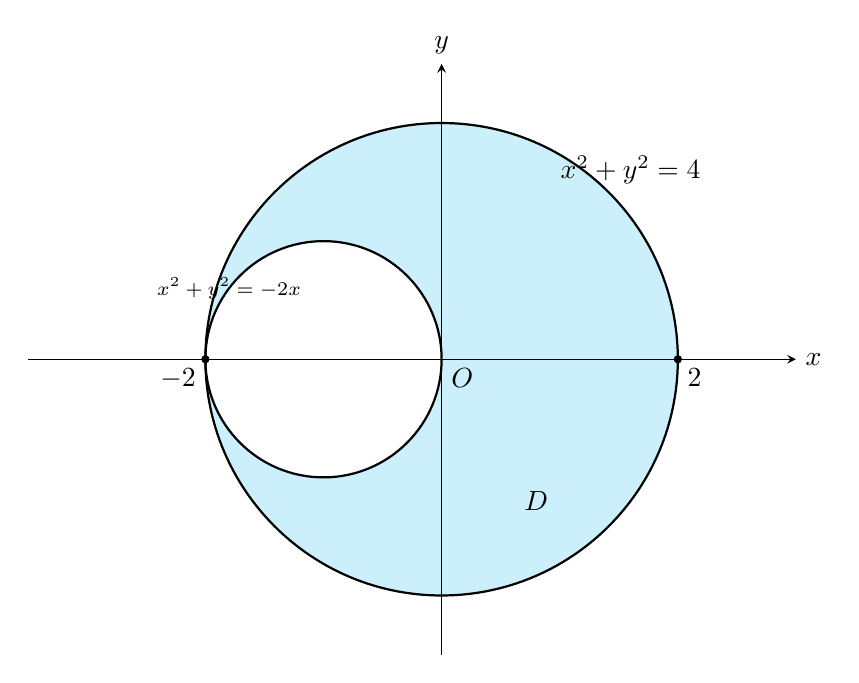
\begin{tikzpicture}[scale=1.5, >=stealth]
    % 填充积分区域 D (大圆内部挖去小圆)
    % 使用 even odd rule 可以完美实现镂空效果
    \fill[cyan!20, even odd rule] (0,0) circle (2) (-1,0) circle (1);

    % 画坐标轴
    \draw[->] (-3.5, 0) -- (3.0, 0) node[right] {$x$};
    \draw[->] (0, -2.5) -- (0, 2.5) node[above] {$y$};

    % 画大圆 x^2 + y^2 = 4
    \draw[thick] (0,0) circle (2);
    \node at (1.6, 1.6) {$x^2+y^2=4$};

    % 画小圆 (x+1)^2 + y^2 = 1 (即 x^2 + y^2 = -2x)
    \draw[thick] (-1,0) circle (1);
    \node at (-1.8, 0.6) {\scriptsize $x^2+y^2=-2x$};

    % 标注原点和关键坐标
    \node[below right] at (0,0) {$O$};
    \fill (2,0) circle (1pt) node[below right] {$2$};
    \fill (-2,0) circle (1pt) node[below left] {$-2$};

    % 标注区域 D
    \node at (0.8, -1.2) {$D$};
\end{tikzpicture}
\end{document}
